\chapter{Nutzerstudie}\label{study}

Wie in der Zielsetzung festgelegt wurde die Usability des digitale Prototypen für die Erstellung, Bearbeitung und Löschung von Feedback 
in einer Nutzerstudie evaluiert. Da im Prototypen zwei unterschiedliche Darstellungsformen für die Feedback implementiert wurden aus die jeweils die Aufgaben: Bearbeitung 
und Löschung von Feedback gelöst werden konnten, kam die Frage auf welche Unterschied Hinsichtlich der Usability zwischen diesen Darstellungsformen festgestellt werden kann. 

Im Kapitel \ref{anlayse_capter} Abschnitt \ref{brand_abschnitt} sowie im Abschnitt \ref{ipi_section} wurden Studien betrachtet welche unterschiedliche Darstellungsformen 
miteinander vergleichen. Auf Grudlaage der Ergebnissen die \citeauthor{Brandenburg2019} in \cite{Brandenburg2019} identifiziert hat: Dass sich die Darstellung als Annotationen 
am Produkt für Vergleichsaufgaben besser eignen, wurden in dieser Studie zwei gerichtete Hypothesen aufgestellt. 
 
\section{Aufbau der Studie}

\textbf{Versuchspersonen}

An der Studie nahmen 12 Versuchspersonen im Durchschnittsalter von 25 Jahren (Standartabweichung 5,1) teil.  Davon waren 4 weiblich und 8 männlich. 
Alle Versuchsteilnehmer waren Studierende. Zehn davon haben im Studiengang Angewandte Informatik, einer im Maschinenbau sowie einer im Film-Regie. 

Drei der Versuchspersonen haben angegeben regelmäßig Erfahrung mit virtuellen Umgebungen zu haben, Fünf haben  Versuchspersonen haben angegeben dass sie, virtuelle Umgebungen schon 
einmal gesehen oder ausprobiert haben.Nur zwei haben angegeben noch keine Erfahrung bisher hatten. 
Acht Versuchspersonen haben angegeben dass sie seit mehr als 3 Jahren Erfahrung mit Smartphones haben die mit dem Betriebssystem Android Betriebssystem betrieben werden. Zwei haben angegeben kein 
Erfahrung mit Android zu haben. 

Vier der Versuchspersonen gaben an etwa ein mal die Woche Feedback zu Produkten in Online Einkaufsportalen zu lesen. Zwei gaben an seltener als einmal im Monat Bewertungen zu Produkten zu schreiben und einer gab
an zwei bis drei mal im Monat Bewertungen zu schreiben. 

Elf Versuchspersonen gaben an dass es Ihnen selten bis gelegentlich schwer falle  bestimmte Stelle oder Position an einem Produkt zu beschreiben oder Beschreibungen von andren zu verstehen. Nur einer gab an mit 
solchen Beschreibungen keine Schwierigkeiten zu haben. 

\textbf{Material: }

Für den Versuch wurde auf einem Smartphone mit der Bezeichnung: Samsung Galaxy S8 durchgeführt. Auf dem Endgerät war das Betriebssystem Android Version 9 installiert. 
Als Produkt wurde das 3D Modell eines Smart Tripelec genommen. Dies ist ein Fahrrad welches im sitzen gefahren werden kann. Abbildung mussnochrein zeigt das verwendete Modell.

\begin{figure}[H]
	\centering 
	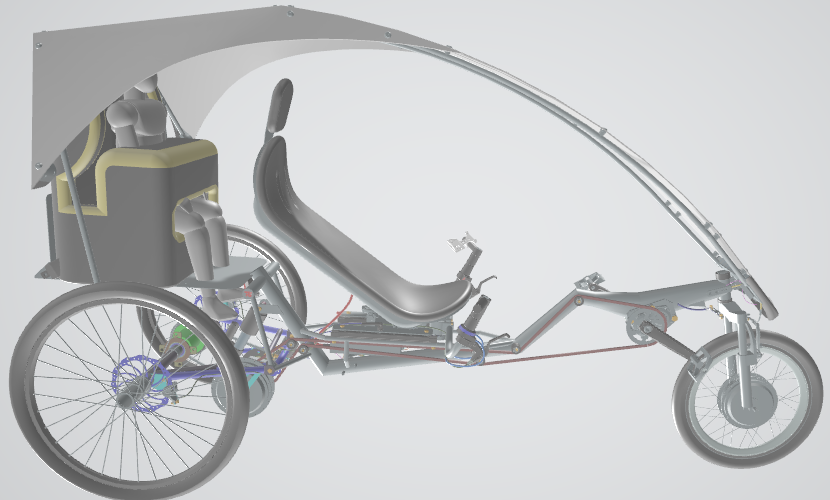
\includegraphics[width=.6\textwidth]{resources/evaluation/SmartTripelec.png}
	\caption{3D Modell Smart Tripelec Quelle: Eigene Abbildung}
	\label{img:mequeMoudul}
\end{figure}

Leider war es aus organisatorischen Gründen nicht das physische Produkt für die Durchführung der Studie zur Verfügung zu haben. So wurde die der Versuch ohne Überlagerung des realen Produktes
an auf dem virtuellen Produkt durchgeführt. 

Das Nutzungserleben (engl. User Experience, kurz UX) wurde nach dem meCUE Fragebogen von \citeauthor{Minge2013} operationalisiert. Dieser Fragebogen ist modular aufgebaut und beinhaltet die Module: 
Produktwahrnehmung, Emotionen, Konsequenzen und das Modul Gesamturteil. Abbildung \ref{img:mequeMoudul} zeigt den Aufbau dieser Module.

\begin{figure}[H]
	\centering 
	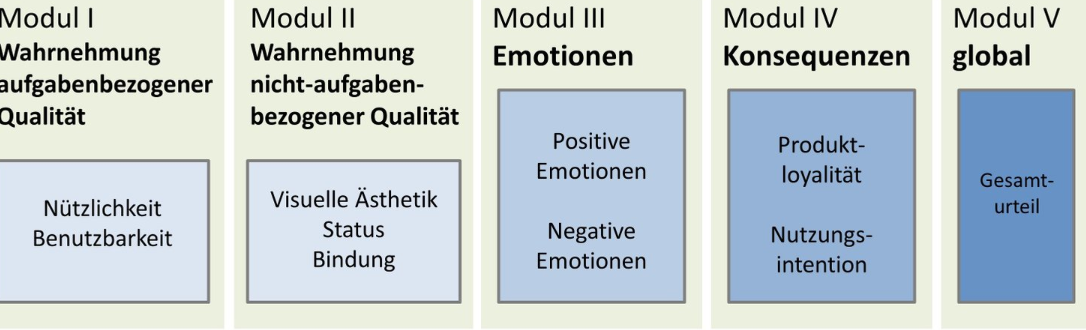
\includegraphics[width=.6\textwidth]{resources/evaluation/meQueModul.png}
	\caption{Darstellungsformen welche in der Studie evaluiert wurden. Quelle: \cite[S.~4]{Minge2013}}
	\label{img:mequeMoudul}
\end{figure} 

In den Modulen M1 bis M3 werden in diesem Fragebogen, Aussagen formuliert deren Zustimmung über ein Likert skaliertes Antwortformat erfasst werden \footnote{Skalenwert von 1 bis 7: ``lehne völlig ab``, ``lehne ab``, ``lehne eher ab``, ``weder
	noch``, ``stimme eher zu``, ``stimme zu``, ``stimme völlig zu``)}\cite{Minge2013}. Im Modul vier kann eine Bewertung von –5 bis 5 (Schrittweite 0,5) als Gesamturteil abgegeben werden. 

\textbf{Unabhängige Variablen:}

Die unabhängige Variablen (UV) ist die Darstellungsform der zu bearbeitenden Feedback. Die Darstellungsform der Feedback wird zweifach gestuft in: 

\begin{itemize}
\item Darstellung der Feedback als Annotation auf dem Produkt sowie
\item Darstellung der Feedback als Listenansicht 
\end{itemize}

\textbf{Abhängigen Variablen}

Objektiv abhänge Variablen sind die Zeiten für die Bearbeitung der Feedback (Zeit vom Start der Anwendung bis zum öffnen des Formulars) für die beiden Darstellungsformen sowie für die Darstellung als Annotation für andren Aufgaben: Erstellung und Löschung von Feedback. Des weiteren zählen die Werte aus dem meQue Fragebogen zu den abhängen Variablen.

\textbf{Prozedur:}

Zunächst haben die Versuchsteilnehmer einen demografischen Fragebogen ausgefüllt. Danach wurde die Studie erläutert und eine Einweisung in die Aufgaben gegeben. 
Dies erfolgte in schriftlicher Form. Die Studien sowie Aufgabenbeschreibungen befinden sich im Anhang. 

Die Aufgaben waren: 

\begin{itemize}
	\item Vier neue Feedback erstellen. Welchen Inhalt die Feedback haben sollten wurde in der Aufgabenbeschreibung vorgegeben. 
	\item Die zuvor erstellten Feedback in der Darstellungsvariante Annotation bearbeiten. In der Aufgabenbeschreibung wurde vorgegeben was sich am Feedback ändern sollte.
	\item Die zuvor erstellten Feedback in der Darstellungsvariante Liste bearbeiten. In der Aufgabenbeschreibung wurde vorgegeben was sich am Feedback ändern sollte.
	\item Die vier Feedback in der Darstellungsvariante Annotation zu löschen.
\end{itemize}

Nach jeder Aufgabenbearbeitung (z. B. nach 4 Iterationen zum Erstellen von Feedback) wurde der MeQue Fragebogen von den Teilnehmern ausgefüllt und die jeweils durchgeführte Interaktion bewertet. 

\textbf{Hypothesen}

Auf Grundlage der Analyse 

H1: Die Darstellung der Feedback als Annotation erhöhen die Nützlichkeit, Benutzbarkeit und Zufriedenheit.\\
\vspace{2mm}H2: Die Zeit in das Formular für die Bearbeitung der Feedback zu gelangen wird mit der Darstellung als Annotation auf dem Produkt weniger Zeit betragen als mit der Darstellung in Listenansicht. 

Beide Darstellungsformen wurden von den gleichen Versuchspersonen durchgeführt.\\ 
Als Signifikanzniveau wurde ($\alpha$)= 0,05 festgelegt. 

\section{Erhebung}

\textbf{Ergebnisse:}

\ac{PTAM}

Abbildung \ref{img:avg_meQue_listAnnotation} zeigt die Mittelwerte für die mit dem meQue Fragebogen bewerteten Produkteigenschaften. 
Sie stellt die Bewertung Produkteigenschaften für die Bearbeitung der Annotation mit der Darstellung als Listenansicht und der Annoation Ansicht nebeneinander. 

\begin{figure}[H]
	\centering
	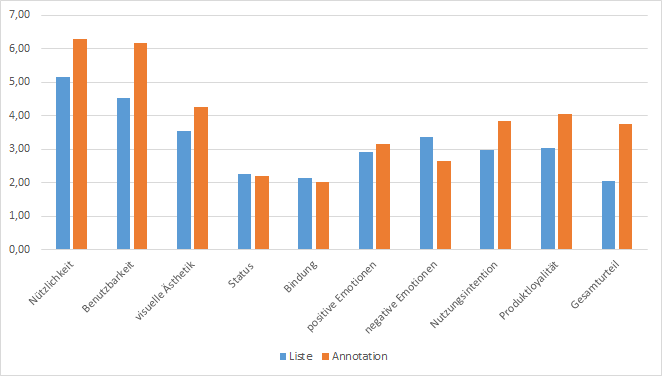
\includegraphics[width=1.0\textwidth]{resources/evaluation/diagrammmittel_vergleich_liste_annotation.png}
	\caption{Vergleich der Mittelwerte aus meQue Fragebogen für Listen vs. Annotation Ansicht \\Quelle:  Eigene Darstellung}
	\label{img:avg_meQue_listAnnotation}
\end{figure}

Auf Abbildung \ref{img:pWerte} sind die p-Werte für Mittelwerte für die Bewertung der Produkteigenschaften zu sehen. Diese wurden in einem T-Test mit ein Signifikanzniveau von Alpha $\alpha$ = 0,05 berechnet. 

\begin{figure}[H]
	\centering
	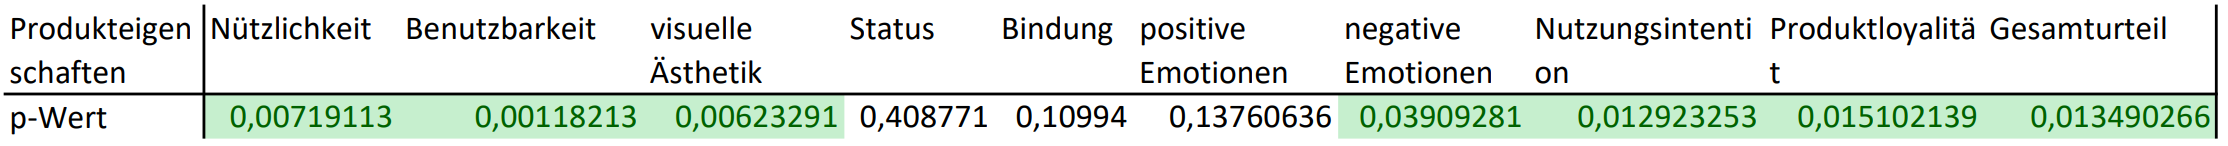
\includegraphics[width=1.0\textwidth]{resources/evaluation/pWerte.png}
	\caption{p-Werte für den Vergleich von meQue Fragebogen Liste vs. Annotation Ansicht\\Quelle:  Eigene Darstellung}
	\label{img:pWerte}
\end{figure}

Abbildung \ref{img:mwListeAnno} zeigt ein Vergleich der Mittelwerte  für die Zeit in Sekunden vom Start der Anwendung bis zum öffnen des Bearbeitungsformulars für die beiden Darstellungsvarianten Liste und Annotation.  

\begin{figure}[H]
	\centering
	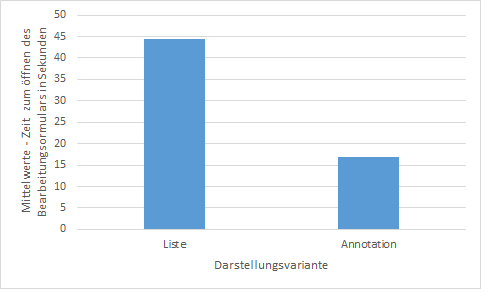
\includegraphics[width=.8\textwidth]{resources/evaluation/mittelwerte_liste_anno.png}
	\caption{Vergleich der Mittelwerte (Liste vs. Annotation) über alle Versuchspersonen und Iterationen. \\Quelle: Eigene Darstellung}
	\label{img:mwListeAnno}
\end{figure}

Hier ergab ein T-Test mit Signifikanzniveau von Alpha $\alpha$ = 0,05 einen p-Wert von 0,064

Auf Abbildung \ref{img:mwUsability} sind die Mittelwerte der Aufgabenbezogenen Produktqualitäten Nützlichkeit (engl. Usability) und Nutzbarkeit (engl. Utility) bewertet nach dem meQue Fragebogen für die 
Aufgaben Erstellung, Bearbeitung und Löschung von Feedback zu sehen. Die Abbildung \ref{img:mwTimes} zeigt die durchschnittlichen Zeiten für diese Aktionen.

\begin{figure}[H]
	\centering
	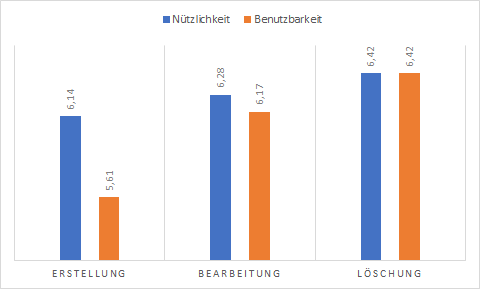
\includegraphics[width=.8\textwidth]{resources/evaluation/MittelWerteUsability.png}
	\caption{Mittelwerte Usability u. Utility für die Aufgaben: Erstellen - Bearbeiten - Löschen in Annotation Ansicht \\Quelle: Eigene Darstellung}
	\label{img:mwUsability}
\end{figure}

\begin{figure}[H]
	\centering
	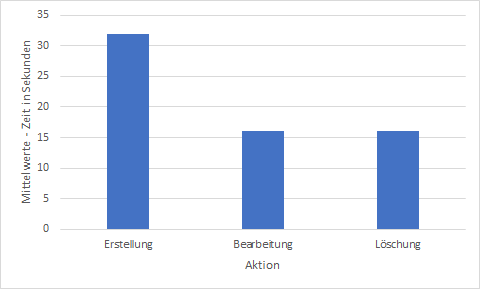
\includegraphics[width=.8\textwidth]{resources/evaluation/mittelwerte_alle_aktionen.png}
	\caption{Mittelwerte der Zeiten für die Aufgaben: Erstellen - Bearbeiten - Löschen in Annotation Ansicht \\Quelle: Eigene Darstellung}
	\label{img:mwTimes}
\end{figure}

\section{Diskussion}

Auf Grundlage der aus Auswertung der erhobenen Daten gewonnenen Erkenntnisse kann folgendes gesagt werden:

Dass in Bezug Aufgabenbezogenen Qualitäten des Prototypen wie die Gebrauchstauglichkeit und Brauchbarkeit die angewandten Methode zum Zeigen und Auswählen auf dem Produkt (\textit{Relativ-Pointing})
sowie die Darstellung der Feedback als Annotation mit Verbindungslinie auf dem Produkt bevorzugt werden können. Sowohl die Mittelwerte des me-Que Fragebogen, in welcher für alle drei Aufgaben mit über 6 bei 
einer Bewertungsskala bis 7 bewertet wurden, als auch die gemessenen Zeiten für diese Aufgabenbearbeitung, mit einem Mittelwert von ca. 30 Sekunden für die Erstellung eines Feedback und 16 Sekunden für die 
Aufgaben Bearbeiten und Löschen bestätigen diese Aussage. 

Die Hypothese H1, trifft auf Grundlage der berechneten p-Werte für die Produkteigenschaften Nützlichkeit, Nutzbarkeit, Visuelle Ästhetik, negative Emotionen, Nutzungsintention sowie Gesamturteil bestätigt werden.
Hypothese H2 jedoch kann mit einem berechneten p-Wert von 0,064 nicht bestätigt werden da dies über dem Signifikanzniveaus von 0,05 liegt. 

Insgesamt kann zusammenfassend gesagt werden dass die Annotation Ansicht für die Aufgaben ein Feedback auf dem Produkt zu Bearbeiten oder zu löschen gegenüber der Listenansicht bevorzugt werden kann. 
Der Prototyp zeigt eine hohe Usability, hat jedoch nach den Ergebnissen des meQue Fragebogens zu urteilen hinsichtlich der Produkteigenschaften Visuelle Ästhetik, positive Emotionen, Status, Nutzungsintention sowie 
Gesamturteil deutliches Verbesserungspotenzial.
 
